% ============================================
% 7 问题4：化学成分关联关系分析
% ============================================
\section{问题4：化学成分关联关系分析}

\subsection{研究方法}

\begin{enumerate}[label=(\arabic*)]
    \item \textbf{CLR 变换}：化学成分数据为成分性数据（各组分之和固定为 $100\%$），直接计算相关性会产生虚假的负相关（闭合效应）。采用 centered log-ratio 变换：
    \begin{equation}
        \text{CLR}(x_j) = \ln\left(\frac{x_j}{g(\mathbf{x})}\right), \quad g(\mathbf{x}) = \left(\prod_{k=1}^{D} x_k\right)^{1/D}
    \end{equation}
    零值处理：以该氧化物最小检出值的一半替代。

    \item \textbf{相关分析}：CLR 变换后计算 Pearson 相关系数，原始数据计算 Spearman 秩相关系数（交叉验证）。

    \item \textbf{类型间差异检验}：Fisher $z$ 变换比较两类玻璃的相关系数差异，$|z| > 2$ 视为显著。

    \item \textbf{风化分层分析}：按 [类型 $\times$ 风化状态] 分 4 层分别计算相关矩阵，比较平均绝对相关系数。
\end{enumerate}

\subsection{高钾玻璃关联特征}

\textbf{最强正相关}（CLR 空间）：

\begin{table}[H]
    \centering
    \caption{高钾玻璃最强正相关对}
    \label{tab:hk_pos_corr}
    \begin{tabular}{l c c}
        \toprule
        \textbf{氧化物对} & \textbf{$r$} & \textbf{含义} \\
        \midrule
        $\text{SiO}_2$ -- $\text{SO}_2$ & $+0.80$ & 风化共富集效应 \\
        $\text{SiO}_2$ -- $\text{SnO}_2$ & $+0.63$ & 风化残留 \\
        $\text{SnO}_2$ -- $\text{SO}_2$ & $+0.49$ & 环境元素共进入 \\
        \bottomrule
    \end{tabular}
\end{table}

\textbf{最强负相关}：

\begin{table}[H]
    \centering
    \caption{高钾玻璃最强负相关对}
    \label{tab:hk_neg_corr}
    \begin{tabular}{l c c}
        \toprule
        \textbf{氧化物对} & \textbf{$r$} & \textbf{含义} \\
        \midrule
        CaO -- SrO & $-0.74$ & Ca-Sr 竞争替代 \\
        $\text{Fe}_2\text{O}_3$ -- $\text{SnO}_2$ & $-0.72$ & 铁与锡互斥 \\
        $\text{K}_2\text{O}$ -- BaO & $-0.64$ & 不同类型助熔剂互斥 \\
        \bottomrule
    \end{tabular}
\end{table}

高钾玻璃中 $\text{SiO}_2$ 与多种微量元素呈强正相关，反映风化淋溶导致 $\text{SiO}_2$ 相对富集的闭合效应。

\subsection{铅钡玻璃关联特征}

\textbf{最强正相关}：

\begin{table}[H]
    \centering
    \caption{铅钡玻璃最强正相关对}
    \label{tab:pb_pos_corr}
    \begin{tabular}{l c c}
        \toprule
        \textbf{氧化物对} & \textbf{$r$} & \textbf{含义} \\
        \midrule
        MgO -- $\text{Al}_2\text{O}_3$ & $+0.56$ & 黏土杂质共现 \\
        $\text{SiO}_2$ -- $\text{Na}_2\text{O}$ & $+0.55$ & 石英-泡碱共存 \\
        $\text{SiO}_2$ -- $\text{Al}_2\text{O}_3$ & $+0.54$ & 石英-黏土矿物伴生 \\
        \bottomrule
    \end{tabular}
\end{table}

\textbf{最强负相关}：

\begin{table}[H]
    \centering
    \caption{铅钡玻璃最强负相关对}
    \label{tab:pb_neg_corr}
    \begin{tabular}{l c c}
        \toprule
        \textbf{氧化物对} & \textbf{$r$} & \textbf{含义} \\
        \midrule
        $\text{Na}_2\text{O}$ -- $\text{P}_2\text{O}_5$ & $-0.71$ & 助熔剂类型互斥 \\
        MgO -- $\text{SO}_2$ & $-0.56$ & —— \\
        $\text{SiO}_2$ -- $\text{P}_2\text{O}_5$ & $-0.54$ & 基体 vs 环境元素 \\
        \bottomrule
    \end{tabular}
\end{table}

铅钡玻璃关联以矿物组合为主（$\text{SiO}_2$-$\text{Al}_2\text{O}_3$-MgO 黏土矿物群），风化影响较轻。

\subsection{类型间关联差异}

共发现 \textbf{18 对}氧化物关联在两类玻璃间存在显著差异（$|z| > 2$）：

\begin{table}[H]
    \centering
    \caption{部分显著差异的氧化物关联对}
    \label{tab:diff_corr}
    \begin{tabular}{l c c c c c}
        \toprule
        \textbf{氧化物对} & \textbf{高钾 $r$} & \textbf{铅钡 $r$} & \textbf{$\Delta$} & \textbf{$z$} & \textbf{解读} \\
        \midrule
        $\text{SiO}_2$ -- $\text{SO}_2$ & $+0.80$ & $-0.41$ & $-1.21$ & $-5.17$ & 最大反转 \\
        $\text{Fe}_2\text{O}_3$ -- CuO & $+0.47$ & $-0.53$ & $-1.00$ & $-3.71$ & 着色剂反向 \\
        $\text{SiO}_2$ -- $\text{Al}_2\text{O}_3$ & $-0.41$ & $+0.54$ & $+0.95$ & $+3.49$ & 基体-杂质不同 \\
        $\text{Fe}_2\text{O}_3$ -- $\text{SnO}_2$ & $-0.72$ & $+0.18$ & $+0.90$ & $+3.65$ & 高钾 Sn 富集风化层 \\
        CaO -- SrO & $-0.74$ & $+0.09$ & $+0.83$ & $+3.49$ & 铅钡无 Ca-Sr 竞争 \\
        \bottomrule
    \end{tabular}
\end{table}

\subsection{风化分层分析}

\begin{table}[H]
    \centering
    \caption{四组风化分层相关分析}
    \label{tab:layer_corr}
    \begin{tabular}{l c c c}
        \toprule
        \textbf{组别} & \textbf{样本量} & \textbf{平均 $|r|$} & \textbf{解读} \\
        \midrule
        高钾-无风化 & 12 & 0.279 & 正常关联强度 \\
        高钾-风化 & 6 & \textbf{0.567} & 风化导致虚假高相关（闭合效应放大） \\
        铅钡-无风化 & 13 & 0.246 & 正常关联强度 \\
        铅钡-风化 & 36 & 0.254 & 风化影响轻微 \\
        \bottomrule
    \end{tabular}
\end{table}

高钾风化组平均 $|r|$ 异常高（0.567），因淋溶后几乎所有元素归零、$\text{SiO}_2$ 占绝对主导，闭合效应被极端放大——这是统计假象而非真实的化学关联增强。

\subsection{结论}

\begin{enumerate}[label=(\arabic*)]
    \item \textbf{高钾玻璃关联网络}：风化淋溶主导——$\text{SiO}_2$ 与全部微量元素正相关（残留效应），元素间竞争替代关系被风化掩盖
    \item \textbf{铅钡玻璃关联网络}：原始矿物组合主导——$\text{SiO}_2$-$\text{Al}_2\text{O}_3$-MgO 黏土群、PbO-BaO 助熔剂群的组内正相关，风化仅部分改变
    \item \textbf{类型间差异}：18/91 对氧化物关联显著不同（$z > 2$），差异核心在于风化对两类玻璃的化学信号重塑程度不同
    \item \textbf{风化效应}：风化在高钾中产生虚假高相关（闭合效应），铅钡中影响较小——进行成分数据相关分析时必须分层处理
\end{enumerate}

\begin{figure}[H]
    \centering
    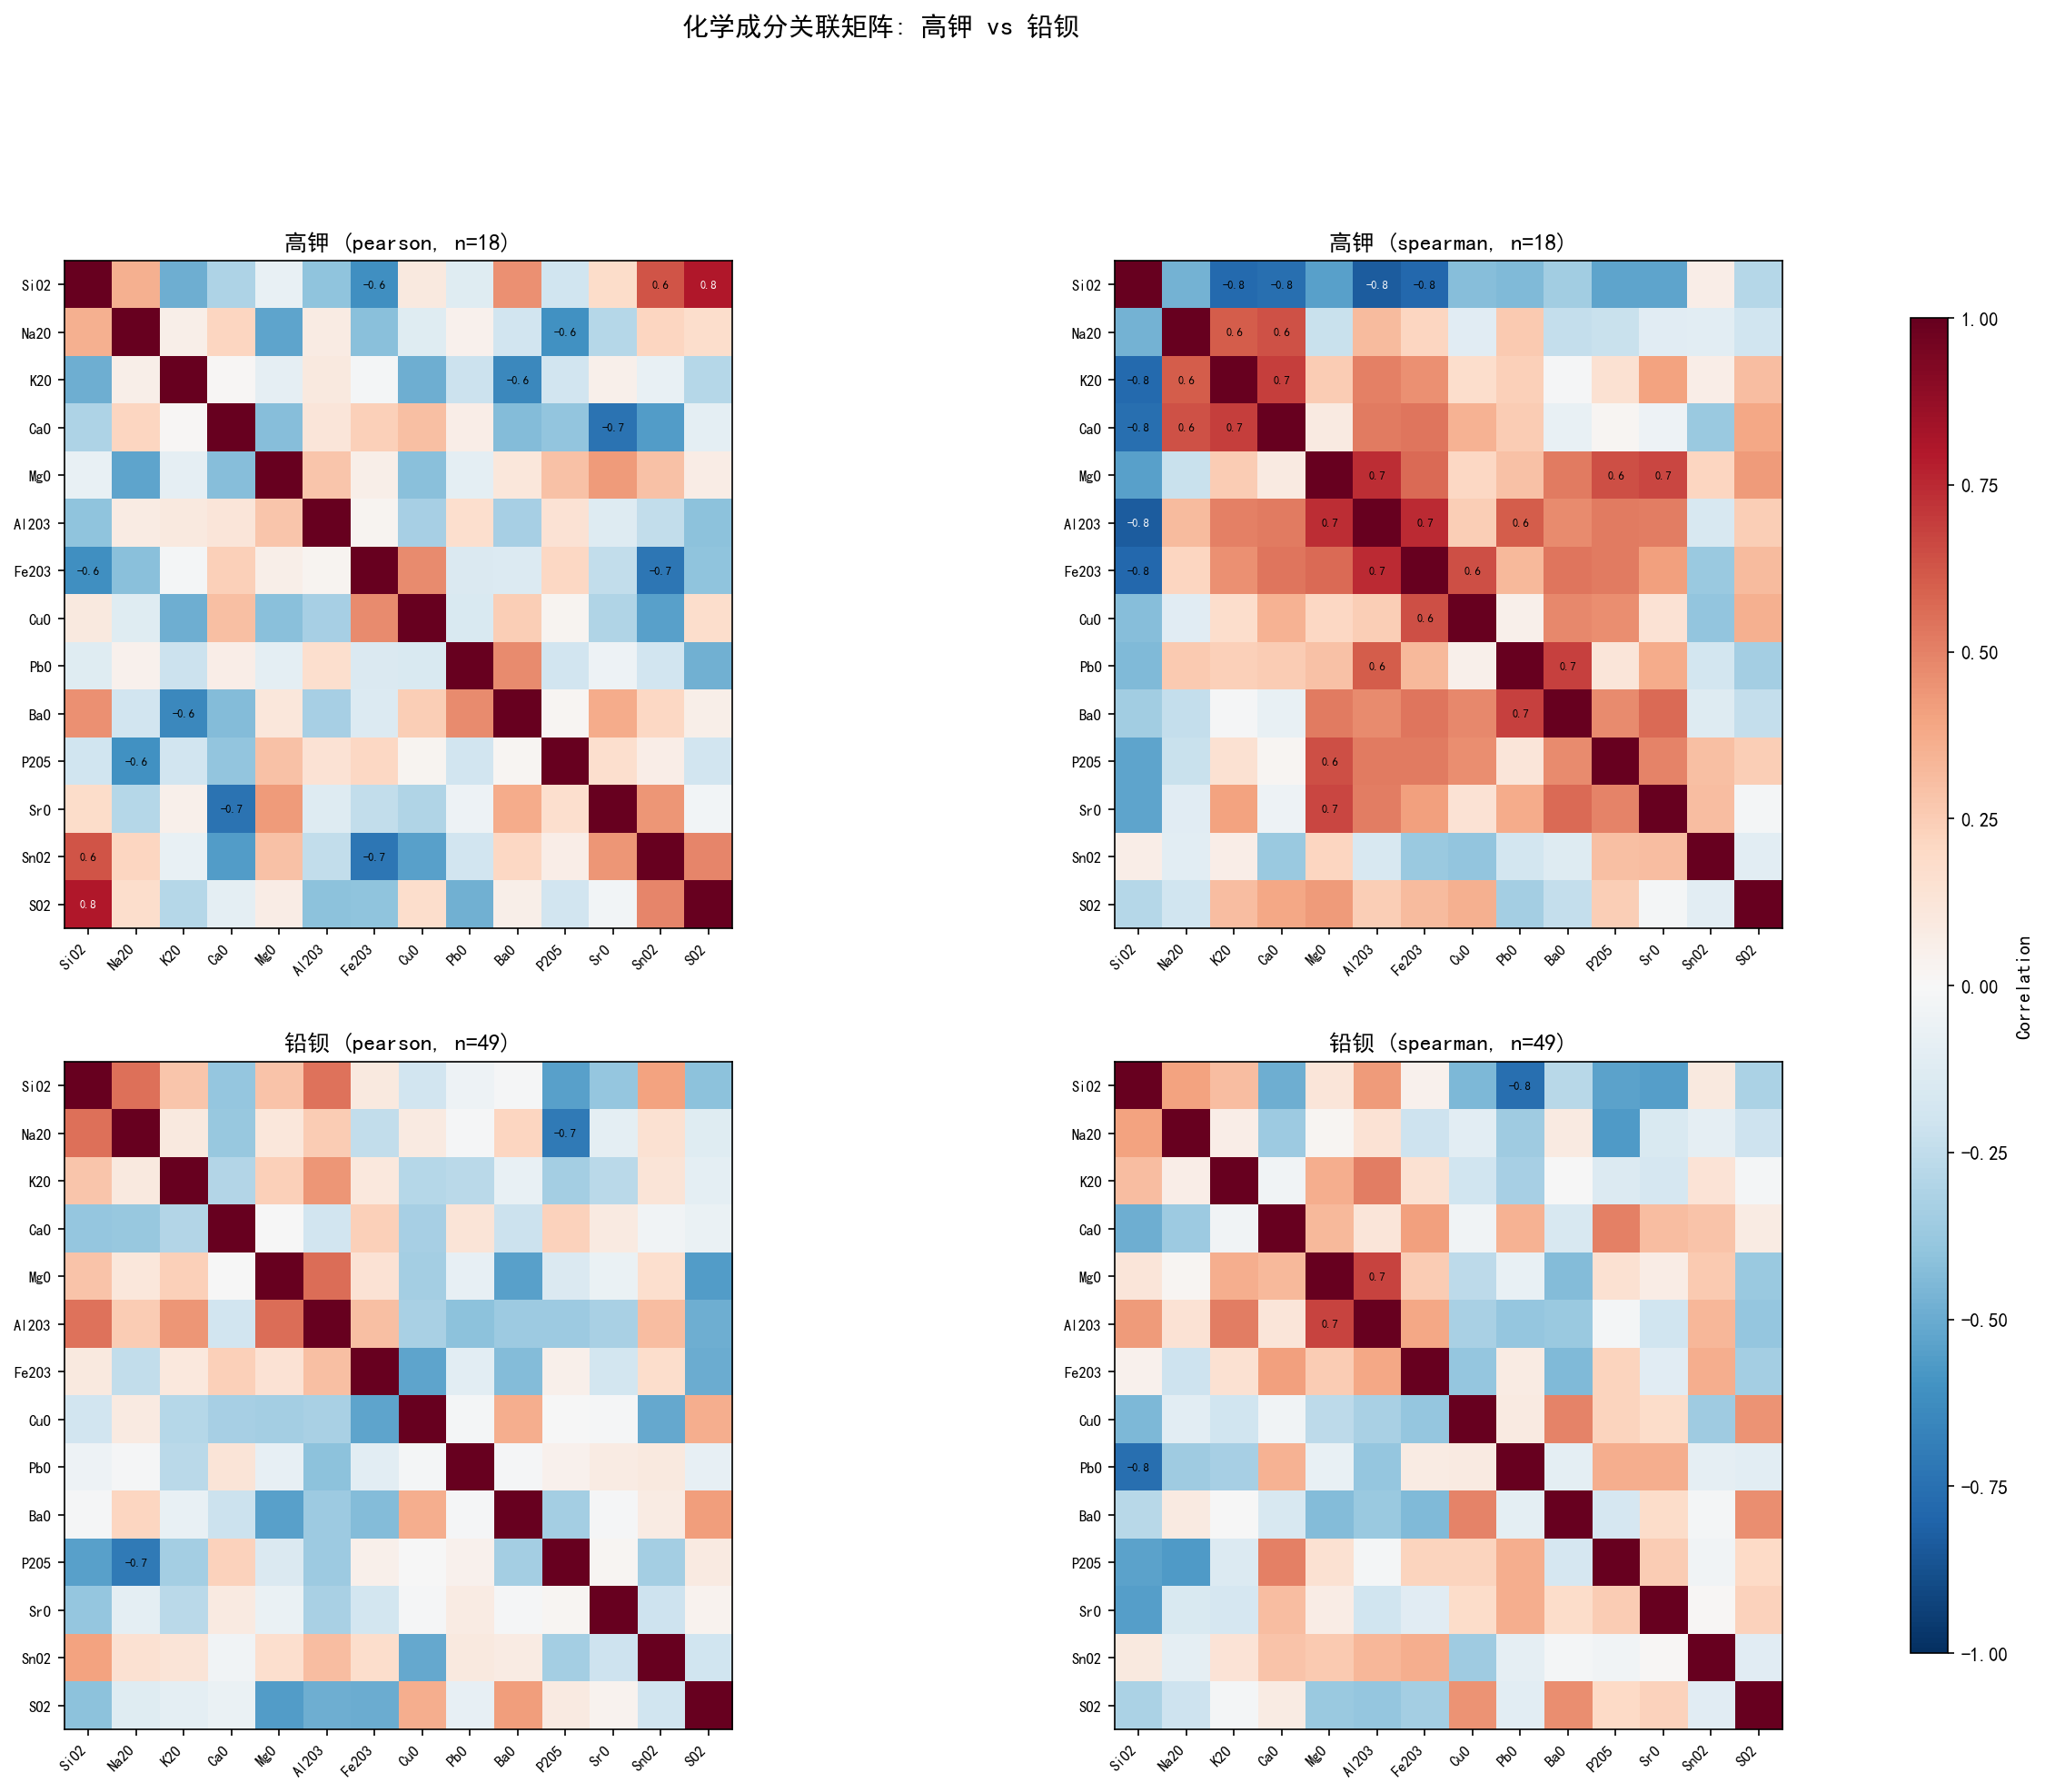
\includegraphics[width=0.95\textwidth]{../analysis/fig4_correlation_heatmaps.png}
    \caption{四组 CLR 相关热力图}
    \label{fig:heatmaps}
\end{figure}

\begin{figure}[H]
    \centering
    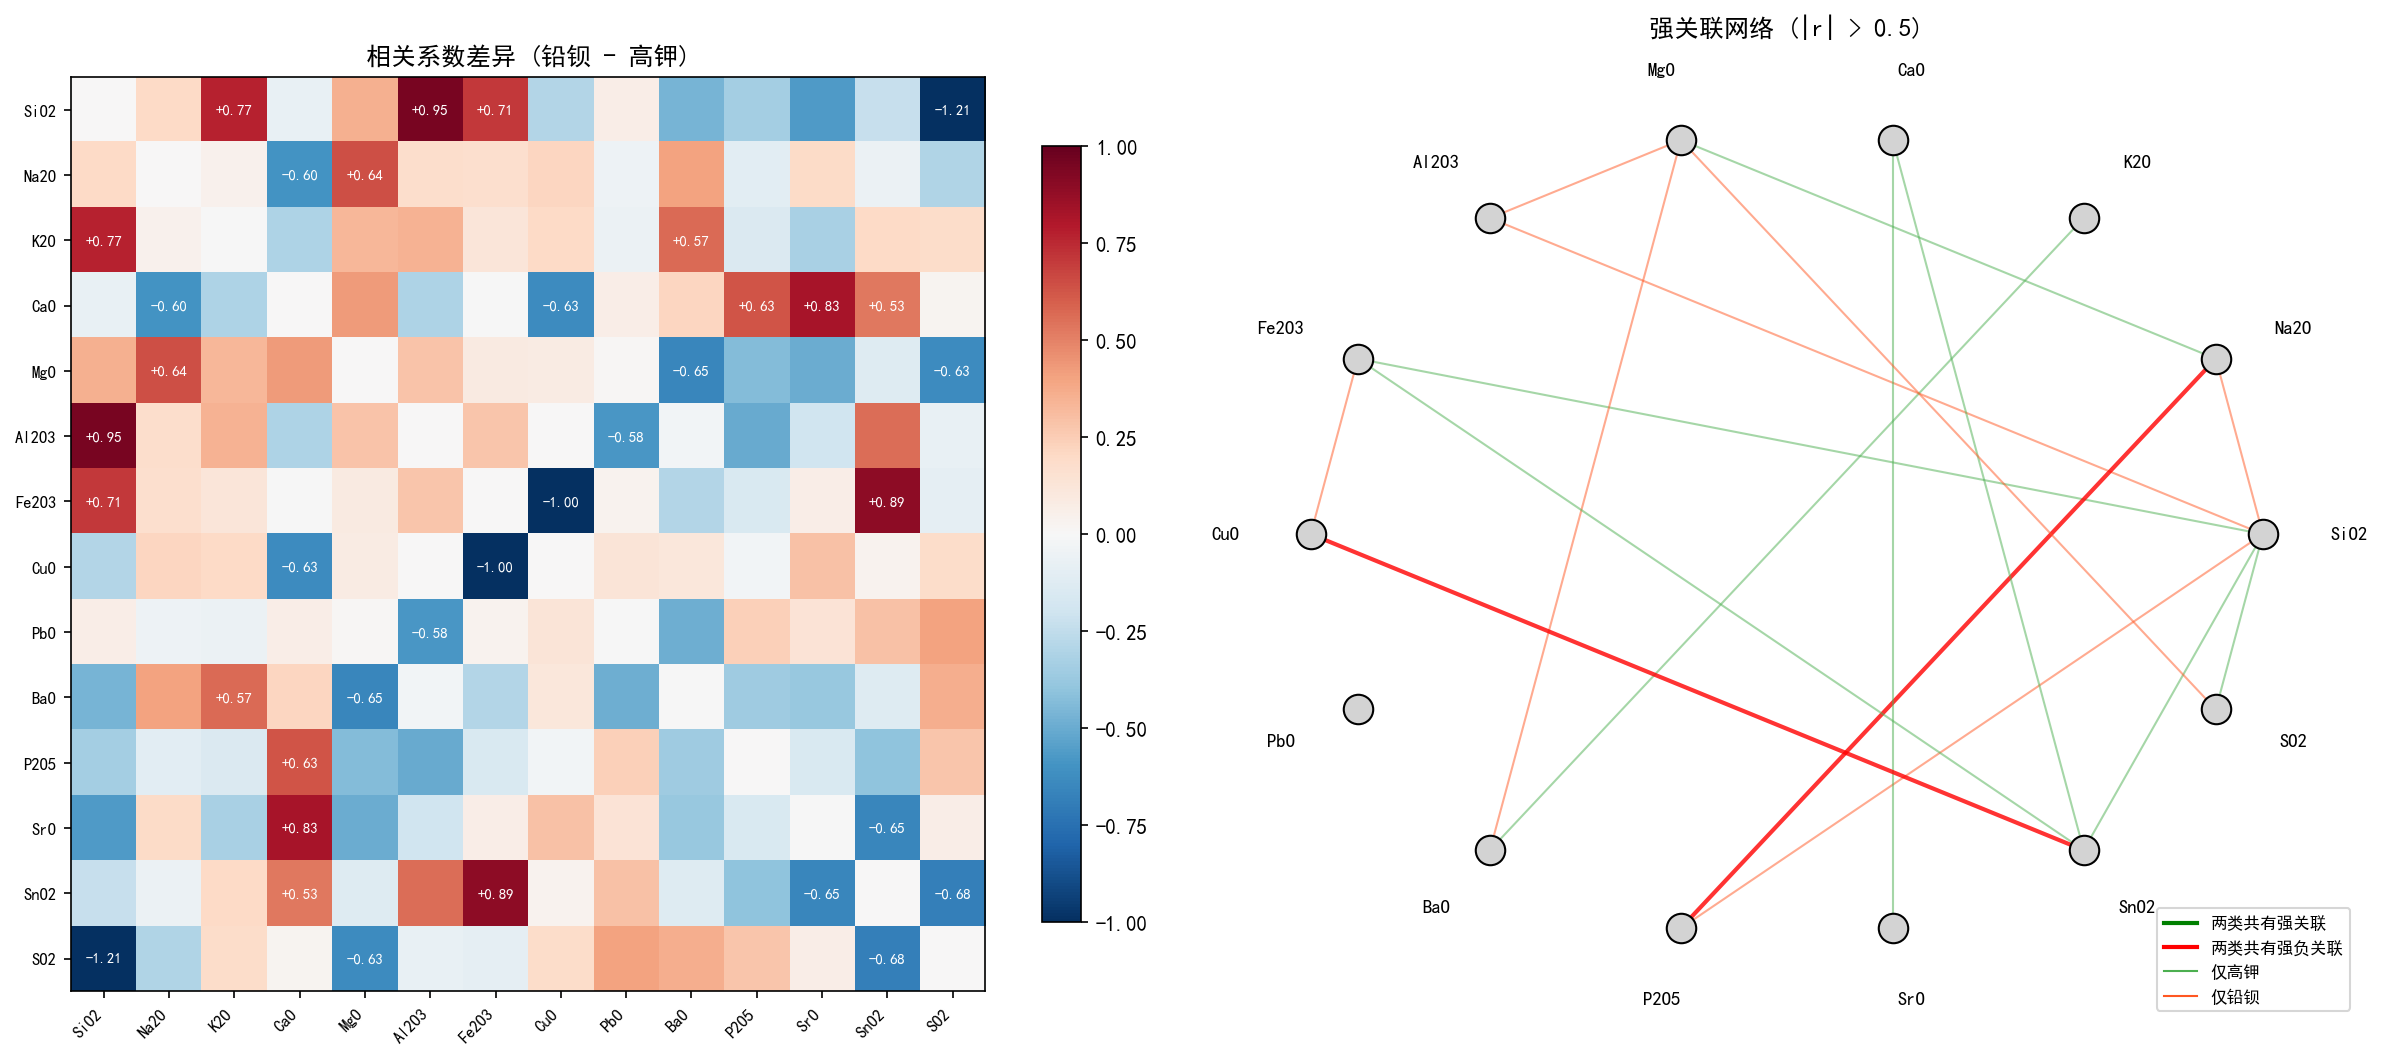
\includegraphics[width=0.95\textwidth]{../analysis/fig4_difference_network.png}
    \caption{类型间关联差异网络图（差异热力图 $+$ 关联网络）}
    \label{fig:diff_network}
\end{figure}
